%
% File acl2018.tex
%
%% Based on the style files for ACL-2017, with some changes, which were, in turn,
%% Based on the style files for ACL-2015, with some improvements
%%  taken from the NAACL-2016 style
%% Based on the style files for ACL-2014, which were, in turn,
%% based on ACL-2013, ACL-2012, ACL-2011, ACL-2010, ACL-IJCNLP-2009,
%% EACL-2009, IJCNLP-2008...
%% Based on the style files for EACL 2006 by 
%%e.agirre@ehu.es or Sergi.Balari@uab.es
%% and that of ACL 08 by Joakim Nivre and Noah Smith

\documentclass[11pt,a4paper]{article}
\usepackage[hyperref]{acl2018}
\usepackage{amsmath}
\usepackage{times}
\usepackage{latexsym}
\usepackage{graphicx}
\usepackage{float}
\usepackage{url}
\usepackage{booktabs}
\usepackage{multirow}

%\aclfinalcopy % Uncomment this line for the final submission
%\def\aclpaperid{***} %  Enter the acl Paper ID here

%\setlength\titlebox{5cm}
% You can expand the titlebox if you need extra space
% to show all the authors. Please do not make the titlebox
% smaller than 5cm (the original size); we will check this
% in the camera-ready version and ask you to change it back.

\newcommand\BibTeX{B{\sc ib}\TeX}

\title{Instructions for ACL 2018 Proceedings}

\author{First Author \\
  Affiliation / Address line 1 \\
  Affiliation / Address line 2 \\
  Affiliation / Address line 3 \\
  {\tt email@domain} \\\And
  Second Author \\
  Affiliation / Address line 1 \\
  Affiliation / Address line 2 \\
  Affiliation / Address line 3 \\
  {\tt email@domain} \\}

\date{}

\begin{document}
\maketitle
\begin{abstract}
  % With development of knowledge representation, research in semantic relatedness measurement continues to make progress.
  % Most of methods for computing semantic relatedness between two words are based on
  % \emph{large corpora} and \emph{lexical databases}.
  % There are only a few of these methods utilize the knowledge graph which contains syntactic and semantic information simultaneously.
  In this paper we focus on computing semantic relatedness getting an approximation to human judgement.
  We utilize the Knowledge Graph(DBPedia) which is derived from wikipedia as the background knowledge.
  For an input pairwise word, we will get two sets of corresponding entities in DBpedia.
  Then we propose a model for extracting a subgraph which contains complete information surrounding two set of entities from DBPedia.
  Then we use a model of knowledge graph embedding to train the subgraph generating high-dimensional vector for each entity and relation. 
  Finally, we get multiple relatedness scores after a join between two set of entities.
  In order to better fit the judgement of human, we utilize a weighted strategy to combine
  multiple relatedness scores of pairwise entities.
  The experiments based on golden dataset for computing semantic relatedness show
  that our model outperform the state-of-the-art model.
\end{abstract}

\section{Introduction}
% problem description: semantic relatedness
Computing semantic relatedness(SR) between two elements(words, sentences,
texts etc.) is a fundamental task for many applications in Natural Language
Processing(NLP) such as lexicon induction\cite{aaai/QadirMGL15}, Named 
Entity Disambiguation\cite{acl/HanZ10}, Keyword Extraction
\cite{ijcai/ZhangFW13} and Information Retrieval\cite{acl/GurevychMZ07}. 
Additionaly, computing semantic relatedness contributes other applications, 
for example, opinion spam problem\cite{www/SandulescuE15}, image classification\cite{iwcs/LeongM11} and so on. 
In this paper we focus on computing semantic relatedness between two 
words in knowledge graph.

It has long been thought that when humans measure the relatedness between
a pair of words, a deeper reasoning is triggered to compare the concepts
behind the words. Many traditional studies on semantic relatedness
utilize different data sources. There are
i) \emph{the large corpora}, such as wikipedia\cite{ijcai/GabrilovichM07},
ii) \emph{the lexical databases}, such as WordNet\cite{acl/Pucher07} or Wikithionary\cite{aaai/ZeschMG08}, 
iii) \emph{the knowledge graph}, such as DBpedia\cite{aaai/NavigliP12} or BabelNet\cite{aaai/NavigliP12}.
With the development of knowledge representation, utilizing knowledge-rich resources to compute semantic 
relatedness is a well-explored line of research. It is known to all that
knowledge graph contains richer syntactic and semantic information than lexical databases,
and more structured knowledge than the large corpora.
On the account of advantages of knowledge graph, we utilize it as background 
knowledge to compute semantic relatedness.

% Knowledge graph can be accessed with powerful query language Sparql in RDF graph.
% As for the methods build on the data soruce, the recent word embedding 
% learning approaches demonstrate their abilities
% to capture syntactic and semantic information, and outperform the
% lexicon-based methods\cite{acl/Pucher07}. 
% Knowledge Graph, as a semantic graph, stores
% vast amount of structured knowledge. 

Recently, there are some researchers having attached importance to measure semantic relatedness
in knowledge graph\cite{acl/IacobacciPN15}, \cite{aaai/NavigliP12}, \cite{aaai/Pirro12}. 
This paper \cite{acl/IacobacciPN15} leveraged entity linking to annotate the dump of wikipedia. Based on this,
the sense-annotated corpus was generated. Then they\cite{acl/IacobacciPN15} used word2vec to
train the sense-annotated corpus and got distributed representation of different 
word senses. This step still needs a significant preprocessing and data transformation efforts. 
As we can see that the author\cite{acl/IacobacciPN15} computed semantic relatedness on account of large corpora.
They just put the knowledge graph on the position of support.
Another paper\cite{aaai/NavigliP12} proposed a knowledge-rich approach to compute multilingual semantic
relatedness which exploited the joint contribution of different languages. Given a pair of words 
in two languages, they\cite{aaai/NavigliP12} utilized BabelNet to collect their translations and computed semantic
relatedness in a variety of languages. Then they combined the empirical evidence from these 
different languages by intersecting their respective graphs.
Another work \cite{aaai/Pirro12} proposed an approach which exploited the graph nature of RDF and SPARQL query
Language to access knowledge graph. It not only obtained the comparable
result with the state-of-art model at that moment, but also avoided the burden
of preprocessing and data transformation.

Though the paper\cite{aaai/Pirro12} avoided a significant preprocessing and data
transformation effort, and develops scalability of their approach while adopting 
the knowledge graph. However, they missed some factors which
might contribute to semantic relatedness measurement. Firstly, given two words
as input, the first step is to find corresponding entities in knowledge
graph. Obviously, there are usually more than one corresponding entities for a single word.
For an input word \emph{car}, for example, we will get \emph{DBPedia:\footnote{http://dbpedia.org/resource}Automobile} and
\emph{DBPedia:Auto\underline{\hspace{0.5em}}Racing} and so on. The work \cite{aaai/Pirro12} losed
sight of the informativeness of the other entities, while they just
consider the entity with the highest rank. Secondly, they \cite{aaai/Pirro12} misseed
some informativeness of \emph{objects} in \emph{triple(subject, prediacte, object)} because their strategy took
the \emph{predicates} into account exclusively based on the TFIDF. This
method ignored the function of \emph{objects} in a semantic triple.

\begin{figure*}
    \centering
    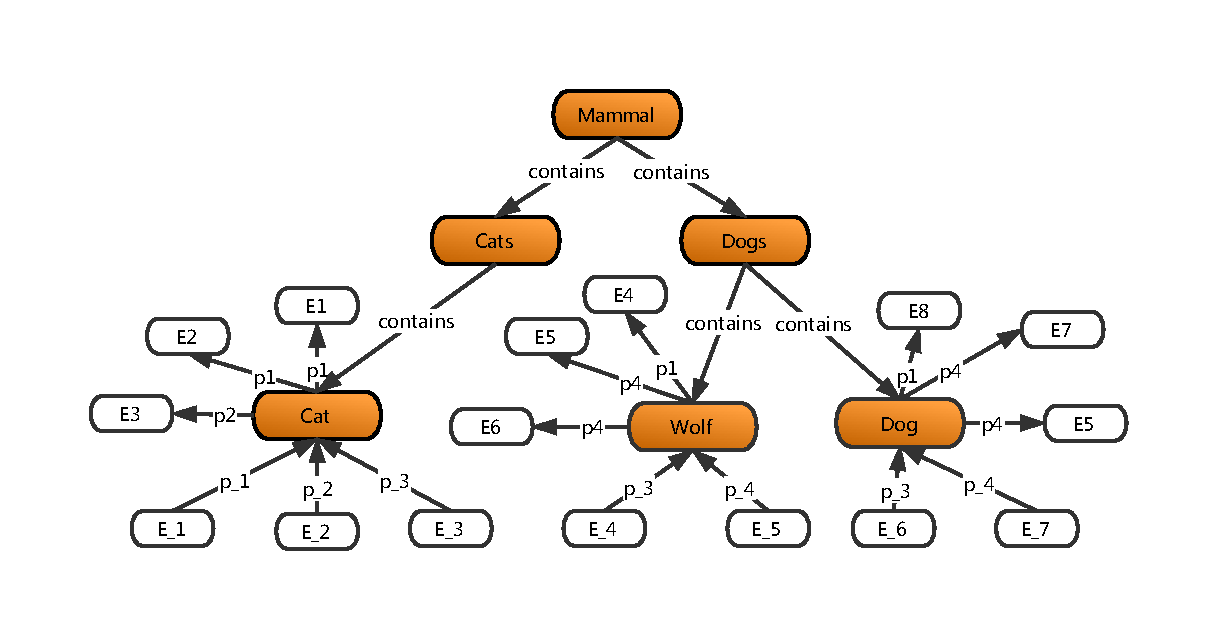
\includegraphics[width=1.1\textwidth]{pic/introduction.pdf}\\
    \caption{Subgraph example in knowledge graph}
    \label{weak1}
\end{figure*}

As show in figure \ref{weak1}, the subgraph contains \emph{Dogs} and \emph{Cats} extracted from
knowledge. We simplify the specific features of \emph{Dogs} and \emph{Cats} to concise symbol shown as $E_i$ in figure. 
We can see that the entity \emph{Cat} plays the role 
of both \emph{Object(Cats contains Cat)} and \emph{Subject(Cat $p_1$ $E_1$)}
in the pattern of triples. The \emph{predicate} which is connected with an entity(Cat)
may be regarded as an outgoing($p_1$) or incoming \emph{predicate}($p_{_1}$).
In the paper\cite{aaai/Pirro12}, the relatedness space for an entity ${E_i}$ is modelled as a 
$k$-dimensional weighted vector \emph{V$_i$}, where each dimension represents
the informativeness of a specific \emph{predicate}.
For example, the weighted vector for \emph{Cat} is 
$[v_{p_1}^o, v_{p_2}^o, v_{p_\_1}^i, v_{p_\_2}^i, v_{p_\_2}^i]$ in which $v_{p_i}^o$ 
means the vector value of outgoing predicate $p_i$ and $v_{p_j}^i$ 
means the vector value of incoming predicate $p_j$.
In this example, from the view of outgoing \emph{predicate} $p_i$, there are three triples
\emph{(Cat $p_1$ $E_1$)}, \emph{(Cat $p_1$ $E_2$)} and \emph{(Cat $p_2$ $E_3$)} which describe the entity \emph{Cat}.
Specifically, in order to compute the vector value of $p_1$,
the way of paper \cite{aaai/Pirro12} in which they got the informativeness of $p_i$ was to count the number
of triples with the form of \emph{(Cat $p_1$ ?)} firstly, then they divided this result
by the total number of triples in which \emph{Cat} appears
((Cat $p_1$ $E_1$), (Cat $p_1$ $E_2$), (Cat $p_2$ $E_3$)), i.e., $v_{p_1}^o$=2/3.
They\cite{aaai/Pirro12} only considered the informativeness of \emph{prediacte},
and ignored the function of a set of specific \emph{objects} in a pattern of triple.
Besides, there is another aspect they have ignored. In this example, for entities $Cat$,
$Dog$ and $Wolf$, let us see the informativeness of prediacte $p_1$. We get
\emph{(Cat $p_1$ $E_1$), (Cat $p_1$ $E_2$), (Wolf $p_1$ $E_4$)} and \emph{(Dog $p_1$ $E_8$)}. 
It is obvious that when they\cite{aaai/Pirro12} computed relatedness between \emph{Cat} and \emph{Wolf}, 
they got the same vector value for predicate $p_1$ both in the aspect of \emph{Wolf} and \emph{Dog}.
In other words, in the dimension of predicate $p_1$ vector between pair (\emph{Cat},\emph{Wolf}) and
(\emph{Cat},\emph{Dog}), they got no difference. Accordingly, they did not distinguish the different
objects for a specific predicate. In order to improve the performance of 
semantic relatedness measurement based on knowledge graph, we propose a threefold model which is shown as follows:

1. For given a pair of words, the first job is to query the corresponding entities. In order to use the
neural network for training the dataset, we also need to construct a graph which contains all related
entities, attributes and relations between the corresponding entity pairs.

2. We use Starspace proposed by Facebook for knowledge graph instead of Word2vec to train the subgraph
extracted from the knowledge graph. Then we can get a distributional representation(vector) for each
entity and predicate. 

3. When we take as inputs a pair of words, we can get two sets of corresponding entities queried from
knowledge graph. Then we can get multiple relatedness scores after a full link between these two sets of entities.
Inspired by \cite{acl/IacobacciPN15}, we utilize an approach to combine the 
relatedness scores as the final semantic relatedness score in knowledge graph.

This paper is organized as follows. We give the related work about semantic relatedness
measurement in section \ref{related-word}. Then we elaborate the threefold model for
computing relatedness scores in section \ref{methodlogy}. Finally, we display detailed
illustrations of experiment results which show that our model outperform the state-of-the-art model.
\section{Related Work}
Computing semantic relatedness(SR) between two elements(words, sentences,
texts etc.) is a fundamental task for many applications in Natural Language
Processing(NLP) such as lexicon induction(\cite{aaai/QadirMGL15}), Named 
Entity Disambiguation{\cite{acl/HanZ10}}, Keyword Extraction
(\cite{ijcai/ZhangFW13}) and Information Retrieval(\cite{acl/GurevychMZ07}). 
Additionaly, computing semantic relatedness contributes other applications, 
for example, opinion spam problem (\cite{www/SandulescuE15}) and so on(+some example). 
In this paper we focus on computing semantic relatedness between two 
words in knowledge graph with neural network.


Semantic measures are mathematical tools used to estimate the strength of the 
semantic relationship between units of language, concepts or instances, through 
a (numerical) description obtained according to the comparison of information 
supporting their meaning. The semantic measures contain semantic relatedness,
semantic similarity, semantic distance. The semantic distance equal to semantic 
unsimilarity. The similarity is only one particular type of relatedness.
Comparison to similarity fails to give a complete view of a relatedness measures.


In this paper we computing semantic relatedness on the account of knowledge
graph. Computational of semantic relatedness is a superset of similarity.
The similarity is only one particular type of relatedness, comparison to
similarity fails to give a complete view of a relatedness measures.

Approaches to measuring semantic relatedness that use lexical
resources (instead of distributional similarity of words, 
e.g. Landauer and Dumais (1997) and Turney (2001)) transform
that resource into a network or graph and compute
relatedness using paths in it. Rada et al. (1989) traverse
MeSH, a term hierarchy for indexing articles in Medline,
and compute semantic relatedness straightforwardly in
terms of the number of edges between terms in the hierarchy.
Jarmasz and Szpakowicz (2003) use the same approach
with Roget’s Thesaurus while Hirst and St-Onge (1998) apply
a similar strategy to WordNet. Since the edge counting
approach relies on a uniform modeling of the hierarchy,
researchers started to develop measures for computing semantic
relatedness which abstract from this problem (Wu and
Palmer, 1994; Resnik, 1995; Leacock and Chodorow, 1998;
Finkelstein et al., 2002; Banerjee and Pedersen, 2003, inter
alia). Those researchers, however, focused on developing
appropriate measures while keeping WordNet as the de facto
primary knowledge source.

\cite{aaai/StrubeP06}
\cite{ijcai/GabrilovichM07}
\cite{www/RadinskyAGM11}

\cite{aaai/Pirro12}
\cite{aaai/NavigliP12}

\cite{acl/IacobacciPN15}

\cite{ijcai/SenJHMOMVWH15} domain specific semantic relatedness 


In this paper we focused on semantic relatedness, which
generalizes similarity by considering not only specialization
relations between words. The application of semantic
relatedness span different areas from natural language processing
(Patwardhan, Banerjee, and Pedersen 2003) to distributed
systems (Pirro, Ruffolo, and Talia 2008). In the Se- ´
8http://relwod.wordpress.com
9http://uniprot.bio2rdf.org/sparql
mantic Web context, some initiatives consider RDF predicates
for vocabulary suggestion (Oren, Gerke, and Decker
2007) while other (Freitas et al. 2011) exploit relatedness
for query answering over Linked Data. However, differently
from REWOrD none of them is specifically focused on computing
relatedness in the Web of Data.
Generally speaking, computational approaches to relatedness
exploit different sources of background knowledge
such as WordNet (e.g., (Resnik 1995; Budanitsky A 2001)),
MeSH (e.g., (Rada, Mili, and Bicknell 1989; Pirro and ´
Euzenat 2010)) or search engines (e.g., (Bollegala, Matsuo,
and Ishizuka 2007; Turney 2001)). Recently, Wikipedia
has been shown to be the most promising source of background
knowledge for relatedness estimation (Gabrilovich
and Markovitch 2007). Therefore we’ll consider approaches
exploiting Wikipedia as baseline for comparison.
WikiRelate! (Ponzetto and Strube 2007), given two words
first retrieves the corresponding Wikipedia articles whose titles
contain the words in input. Then, it estimates relatedness
according to different strategies among which comparing
the texts in the pages or computing the distance between
the Wikipedia categories to which the pages belong.
Explicit Semantic Analysis (Gabrilovich and Markovitch
2007) compute relatedness both between words and text
fragments. ESA derives an interpretation space for concepts
by preprocessing the content of Wikipedia to build
an inverted index that for each word, appearing in the corpus
of Wikipedia articles, contains a weighted list of articles
relevant to that word. Relevance is assessed by the
TFIDF weighting scheme while relatedness is computed by
the cosine of the vectors associated to the texts in input.
WLM (Milne and Witten 2008) instead of exploiting text
in Wikipedia articles, scrutinizes incoming/outgoing links
to/from articles. WikiWalk (Yeh et al. 2009) extends the
WLM by exploiting not only link that appear in an article
(i.e., a Wikipedia page) but all links, to perform a random
walk based on Personalized PageRank.
The most promising approach, in terms of correlation, is
ESA. However, ESA requires a huge preprocessing effort to
build the index, only leverages text in Wikipedia and does
not consider links among articles. Therefore, it may suffer
some problems when the amount of text available is not large
enough to build the interpretation vectors or when changing
the source of background knowledge.
\section{Methodlogy}
\label{methodlogy}
In order to compute semantic relatedness of a pair of words, we propose a model which is
threefold. 
For a given pair of words, we first query the corresponding entities in knowledge graph.
We need to construct a specific graph which contains all related entities and attributes between the 
corresponding entity pairs. Then we use \emph{Starspace}\cite{corr/Ledell17} to train the constructed 
graph. For each entity and relationship, this method produces a representation of vector.
In our method, we use cosine function to compare vectors corresponding to word pairs and get the relatedness scores.
Besides, in the query step, we would get several corresponding entities for an input word. Inspired by
the SenseEmbed\cite{acl/IacobacciPN15}, we combine the relatedness scores computed from the multiple pairs of entities 
as the final measure sorce between two words.

% Please add the following required packages to your document preamble:
% \usepackage{booktabs}
\begin{table*}[]
    \small
    \centering
    \caption{Query Entities (\emph{DBPedia:} equals \emph{http://dbpedia.org/resource/})}
    \label{entities}
    \renewcommand\arraystretch{1.6}
    \setlength{\tabcolsep}{0.8mm}{
    \begin{tabular}{llclc}
    \toprule
    \textbf{Words}  & automobile                                               & \textbf{Refcount} & car                                      & \textbf{Refcount} \\ \hline
    \textbf{Entity} & DBPedia:Automobile                   & 5096     & DBPedia:Automobile   & 5096     \\ \hline
    \textbf{Entity} & DBPedia:Auto\_racing                 & 2885     & DBPedia:NASCAR       & 4317     \\ \hline
    \textbf{Entity} & DBPedia:Ferry                        & 2501     & DBPedia:Tram         & 3988     \\ \hline
    \textbf{Entity} & DBPedia:Internal\_combustion\_engine & 1639     & DBPedia:Auto\_racing & 2885     \\ \hline
    \textbf{Entity} & DBPedia:Gasoline                     & 1486     & DBPedia:Ferry        & 2501     \\ \hline
    \end{tabular}    
    }
\end{table*}

\subsection{Construct graph}
\label{sec:construct graph}
Our aim is to compute the semantic relatedness between a pair of words. The process of relatedness measure
needs complete and ample background knowledge which can be gathered from knowledge graph, such as
DBPedia\footnote{http://wiki.dbpedia.org/}, 
YAGO\footnote{https://www.mpi-inf.mpg.de/departments/databases-and-information-systems/research/yago-naga/yago} etc.
The first problem we face is how to obtain knowledge which is associated with given words from knowledge graph. 
In our model, we utilize the DBPedia as our knowledge base to gather corresponding entities triggered by the given words.
We rely on lookup service\footnote{http://lookup.dbpedia.org/api/search/KeywordSearch} that is provided by DBPedia to achieve this object. 
We use $W_{w_i}$ to denote the set of corresponding entities in knowledge graph when we complete a query by word $w_i$.
Then we get $W_{w_i}=\{E_1,...,E_k\}$ where $E_i$ is the $i_{th}$ query entity associated with the given word.
As show in Table \ref{entities}, for a given word pair \emph{(automobile,car)}, 
we can get the appropriate entities which are described as URIs in DBPedia. 
These URIs describe entities so accurate that we can access knowledge graph using powerful
query language SPARQL\footnote{https://www.w3.org/TR/sparql11-overview/} to get everything we want.

% sparql query norm for graph construction

An entity can be surrounded by entities as well as attributes. There is an example to illustrate this structure
in knowledge graph. Suppose that there is a person \emph{A}, his age is \emph{24}. His name is \emph{"John A"}.
He has a friend called person \emph{B}. This person \emph{B} is an Entity surrounding the \emph{A}.
Then the number \emph{24} and the literal \emph{"John A"} are not entities in knowledge graph,
but all are the attributes surrounding this person \emph{A}.
We can use the URIs shown in table\ref{entities} to access knowledge graph with the help of SPARQL. Next we need to construct a subgraph 
that contains all related entities, attributes and relations between the corresponding entity pairs. Inspired by BabelRelate!\cite{aaai/NavigliP12},
we propose a modified method to get our semantic subgraph. We get query sets of entities $W_{w_1}$ and $W_{w_2}$ individually
by words $w_1$ and $w_2$. Then we select the subgraph which contains all the paths which connect entities in
$ENT = W_{w_1} \cup W_{w_1}$. Besides, this subgraph also contains all attributes for each entity in $ENT$. We do 
this by building a directed graph ${G = (V, E)}$ which contains all relevant information which describes
the entities set.

i) We define the set $V$ in $G$ as $V:=ENT$ first. 
The size of set $V$ is not fixed. It would be extended in the following steps.
As for the set $E$, we initialize it as empty, i.e., $E:=\emptyset$.

ii)The goal of our method is to get the precise vector representations for entities,
that requires more complete information which surround the entities.
Accordingly, for a specific entity, we not only need to consider its neighbor entities or attributes, but also
need to find all paths which connect the nodes in $V$. 
It is known to all, the shorter length of paths between two entities, the more relative these entities are.
We firstly get the one-hop neighbors for each $v \in V$. 
Secondly, we adopt Depth-First Search(DFS) to go through the knowledge graph. Every time we find a node
$v^{'} \in V$ but $v \ne v^{'}$ along a path($v, v_1, v_2,...,v_n, v^{'}$), we add all intermedia 
nodes and edges in this path to $G$, i.e., $V:=V \cup \{v_1, ..., v_n\}$, 
$E:=E \cup \{(v, v_1), ..., (v_n, v^{'})\}$.

iii) Next, we get all relevant attributes which are described as literal, number or something 
else special symbol in knowledge graph. For one entity $v_i \in V$, we collect all the one-hop attributes 
$\{a_1, a_2, ..., a_k\}$. Then we have $V:=V \cup \{a_1, ..., a_k\}$ and
$E:=E \cup \{(v_i, a_1), ..., (v_i, a_k)\}$ ($v_i \in V$).

By this way, we extract a subgraph from DBPedia which consists of the relevant information which describes
the pair of entities.

\subsection{Embedding for Subgraph}
\label{sec:train}
The constructed graph is fundamentally a multi-relational graph in which an entity is described by a set of discrete
\emph{entities} and \emph{attributes}. Fortunately, there have been an excellent work proposed by Facebook AI Research,
\emph{StarSpace}\cite{corr/Ledell17}. The model works by embedding those entities comprised of discrete features and
comparing them against each other. In this section, we introduce the basic contents of \emph{StarSpace} briefly and 
elaborate how we utilize this model to get the vector representation of entities and relations. \emph{StarSpace} is available as
an open-source project at github\footnote{https://github.com/facebookresearch/StarSpace}.

In \emph{StarSpace}, to train our model, we need to compare entities which are described by a set of discrete
\emph{entities} and \emph{attributes}. Specially, there is the following loss function in $StarSpace$:

\begin{small}
    \begin{equation}
        \nonumber
        \label{starspace_formula}
        \sum_{\substack{(a,b) \in V^+\\ b^- \in V^-}}L^{batch}(sim(a,b),sim(a,b_1^-),...,sim(a,b_k^-))
    \end{equation}
\end{small}
In our problem, the input data is a graph of $(h, r, t)$ triples, consisting of a head entity $h$, 
a relation $r$ and a tail entity $t$.
Following the original paper which describes $StarSpace$, there are several explanations for this loss function:

1) The positive entity pair (a,b) comes from the set $V^+$ sampled from constructed graph $G$. 
In our problem, the input is a group of triples $(h, r, t)$. In order to make our input fit
the sample batch $(a, b)$, we need to select uniformly at random to get positive sample $V^+$ in two strategies:
(i)$a$ consists of the bag of features $h$ and $r$, while $b$ consists only of $t$; 
(ii)$a$ consists of $h$, and $b$ consists of $r$ and $t$. 

2) Negative entities $b^-$ are sampled from the set of possible entities $V^-$.  
StarSpace utilizes a $k$-negative sampling strategy\cite{corr/Mikolov13} to select $k$ negative pairs for each batch update. 
They select randomly whithin the set of entities that can appear in the second argument of the similarity function.

3) The selection of function $sim(.,.)$ is designed as a hyper-parameter: cosine similarity and inner product.
In our problem, we adopt cosine similarity for the model as the cosine works better than inner product for
larger dataset. This situation is mentioned in the paper of StarSpace.

4) The loss function $L_{batch}$ compares the positive pairs $(a,b)$ with the negative pairs $(a, b_i^-)$, $i=1,...,k$.
It is also optional between margin ranking loss and negative log loss of softmax. All experiments in $StarSpace$ show
the former performed on par or better. Thus we use margin ranking loss as our loss function for computing semantic relatedness.

5) The method optimization inherit the strategy of stochastic gradient descent(SGD) used in $Starspace$. Each SGD step is one
sampling from $V^+$ in the outer sum.

As a result, we take the constructed graph $G$ of $(h, r, t)$ triples as inputs for the training model.
For each entity and relation in graph $G$, there is a fixed-length vector which can
then be used to compute semantic relatedness via cosine function.

%(Experiments:K-sample,dim of vector,epochs)
% \cite{aaai/BordesWCB11}


\subsection{Semantic Relatedness Measure}
\label{sec:measure}
For a given pair of words($w_m$, $w_n$), we get ($W_{w_m}$, $W_{w_n}$), and $W_{w_m}=\{E_m^1,E_m^2...,E_m^k\}$,
$W_{w_n}=\{E_n^1,E_n^2,...,E_n^k\}$. Then for each entity $E_m^i$ in $W_{w_m}$, we will get learnt embedding vector
$\overrightarrow E_m^i$.
Note that, there might be different number of entities associated with the given
word. We just consider the top-$k$ entities in each entities set. An analysis of the impact of $k$ is
given in section of experiments.

For a pair ($w_1$, $w_2$), we compute semantic relatedness between their corresponding entities. After that, we
get $k*k$ relatedness results where $k$ is number of entities queried from knowledge graph.
The task which combines multiple semantic measurement is similar with the work in SenseEmbed\cite{acl/IacobacciPN15}.
The author captureed the different meanings of a word and transformed word embedding to the sense level.
They utilized the weighted combination of comparison in sense level which achieved a high correlation coefficient.
In our work, the multiple-pair entities produce different semantic measurement. Traditional work only considers the
the relatedness measurement of closest objects. If we only utilize closest combination, the contributions of the other
entities would be ignored. Following the work in SenseEmbed, we combine all those relatedness
results reasonably to get more human-like measurement.

1) For two entities $E_1$ and $E_2$, we utilize cosine function to compute the
distance between two embedding vectors($\overrightarrow E_1$, $\overrightarrow E_2$):

\begin{small}
    \begin{equation}
        \label{cos}
        \nonumber
        Cos(\overrightarrow E_1,\overrightarrow E_2) = \frac{\overrightarrow E_1 \cdot 
        \overrightarrow E_2}{\left \| \overrightarrow E_1 \right \|\left \| \overrightarrow E_2 \right \|}
    \end{equation}
\end{small}

2) Following SenseEmbed, we take two strategies to compute semantic relatedness between given
words $w_1$ and $w_2$ for comparison. One is conventional approach \cite{BudanitskyH06} which considers just the closest entities
among multiple vector pairs. There are $W_{w_1}$ and $W_{w_2}$ represent two entities sets associated with two
input words $w_1$ and $w_2$. $\overrightarrow E_i$ is the learnt embedding vector of entity $E_i$. We can get the
formalization for this strategy.

\begin{small}
    \begin{equation}
        \label{cos}
        \nonumber
        Rel_{closest}(w_1, w_2) = \max \limits_{\substack{E_1 \in W_{w_1} \\ E_2 \in W_{w_1}}}
        Cos(\overrightarrow E_1,\overrightarrow E_2)
    \end{equation}
\end{small}
However this relatedness measurement approach misses contributions of the other entities.
In fact, psychological studies suggest that humans, while comparing similarity between a pair of words, consider
different meanings of two words but not only the closest pairs\cite{Tversky77}. This claim can be directly popularized to compute
relatedness between words. There usually are various meanings for a single word. Analogously we can query multiple
entities associated with the word from knowledge graph. Only consider the entities pair which have the closest distance
would not be conforming with the way of human thinking.

There is another strategy for computing semantic relatedness, called \emph{weighted}, in which
we consider the contributions of different entities associated with given words. The contributions are
scaled according to how they relative to the words. Fortunately, the lookup services of DBPedia can
return a list of ranked DBpedia resources for a search string or a single word. There is a specific label called
$Refcount$ that count the number of Wikipedia page inlinks for a resource. This number is required for ranking.
We can utilize this number to estimate the dominance of each specific entity resource in knowledge graph.
To this end, we use an operation of normalization. For each entity $E \in W_{w_i}$, we get the dominance of
$E$ by dividing the value of $Refcount$ by the sum of all $Refcount$ value of entities in  $W_{w_i}$:

\begin{small}
    \begin{equation}
        \label{cos}
        \nonumber
        d(E) = \frac{refcount(E)}{\sum_{{E}'\in W_i} refcount({E}')}
    \end{equation}
\end{small}

Besides, those entities which are closer would play a more important role in computing semantic relatedness.
Following the SenseEmbed, we model this by biasing the relatedness computation towards closer entities through a power function with
parameter $\alpha$. The relatedness of a pair of words $w_1$ and $w_2$ is computed by using $weighted$ strategy:

\begin{small}
    \begin{equation}
        \begin{split}
        \label{cos}
        \nonumber
        Rel_{weight}&(w_1, w_2)=\\ 
        &\sum_{E_1 \in W_1}\sum_{E_2 \in W_2}d(E_1)d(E_2)Cos(\overrightarrow E_1,\overrightarrow E_2)^\alpha 
        \end{split}
    \end{equation}
\end{small}

In this strategy, we given the entity pairs which is closer a more important role to determine the final semantic relatedness
score. Experiments in below show that the $weighted$ strategy outperforms the $closest$.
% \begin{small}
%     \begin{math}
%         \label{cos}
%         \nonumber
%         Dis(E_1,E_2)
%         =\lambda Cos(\overrightarrow E_1,\overrightarrow E_2) + (1-\lambda)\frac{1}{path(E_1, E_2)}
%     \end{math}
% \end{small}


% \begin{small}
%     \begin{equation}
%         \label{cos}
%         \nonumber
%         Cos^*(\overrightarrow E_1,\overrightarrow E_2)=
%         \begin{cases} 
%         Cos(\overrightarrow E_1,\overrightarrow E_2) \times \beta, &if(s_1, s_2) \in E\\
%         Cos(\overrightarrow E_1,\overrightarrow E_2) \times \beta^{-1}, &otherwise
%         \end{cases}
%     \end{equation}
% \end{small}
\section{Experiment}
In this section, we conduct extensive experiments on different datasets which
contain the semantic measurement by human perceptions. We compute the Spearman
correlation coefficient between results of experiments and scores of human judgement
to evaluate the performance of our model. The model is implemented on 
cpu Core-7-7700K@4.20GHz$\times$8 machine with 16GB memory and ArchLinux platform.
 
\subsection{Dataset}
To evaluate models for semantic relatedness measurement, a common approach is to compare
the scores from the model and the scores provided by humans performing the same task.
This approach provides a model-independent way for evaluating measures of relatedness.
A good number of datasets record the scores of human quantitative judgement
for semantic relatedness such as \emph{MC-30}\cite{MC30/Miller02}, \emph{RG-65}\cite{RG65/RubensteinG65}, 
\emph{REL-122}\cite{acl/SzumlanskiGS13}, \emph{MEN}\cite{MEN/BruniTB14}, 
\emph{YP-130}\cite{YP130/Yang06verbsimilarity}, \emph{WS}\cite{ws/AgirreAHKPS09},
\emph{wordsim-353}\cite{wordsim353/FinkelsteinGMRSWR02}
and so on. Some of these datasets are established with the measurement of 
similarity called \emph{similarity dataset}. Some others are \emph{relatedness dataset}.
Note that all these datasets are English-language words.

1)\emph{similarity dataset}:
\emph{MC-30}, \emph{RG-65}, \emph{YP-130} and \emph{wordsim-353} are all established for computing similarity.
\emph{RG-65} is the classical similarity dataset which contains 65 pairs of words.
\emph{MC-30} contains 30 pairs of words and is the subset of \emph{RG-65}.
\emph{YP-130} is established for computing verb similarity which contains 130 pairs of verb.
\emph{wordsim353} contains two parts that are annotated by different groups of annotators.
The first set (set1) contains 153 word pairs along with their similarity scores assigned by 13 subjects. 
The second set (set2) contains 200 word pairs, with their similarity assessed by 16 subjects.
All these above are mere similarity datasets which just consider a particular case of relatedness.
There is another hybrid dataset \emph{WS} contains two sets of English words pairs along
with human-assigned similarity and relatedness judgements, called \emph{WS-sim} and \emph{WS-Rel} separately.
\emph{WS-sim} contains 203 pairs of words along with similarity judgement,
and \emph{WS-rel} contains 252 along with relatedness judgement.

2)\emph{relatedness dataset}:
Compared to the similarity datasets, there are a small number of relatedness datasets such as
\emph{WS-Rel}, \emph{MEN} and \emph{REL-122}. \emph{WS-Rel} contains 252 pairs of words with
human-assigned relatedness judgements. \emph{MEN} contains 3000 pairs of words which do not
instruct the subjects about the difference between similarity and relatedness. 
Due to the great number of human-assigned relatedness judgements, \emph{MEN} can
be used to train and test computer algorithms implementing semantic similarity or relatedness measures.
We would not consider this collection in our experiments because of the illegibility of semantic measurement.
Another dataset \emph{REL-122} is a new relatedness norm, and contains a set of human-assigned relatedness scores
for 122 pairs of nouns.

The difference between similarity dataset and relatedness dataset is how human assign the score for a
given pair of words. A common example is the pair of words \emph{"wheels-car"}. The \emph{wheels} is more related
with the \emph{car}, but they are dissimilar. The paper \cite{acl/SzumlanskiGS13} created two additional experimental 
conditions in which subjects evaluated the relatedness of noun pairs from the similarity dataset \emph{MC-30}. We select 
ten pairs of words shown in table \ref{mc}. 

\begin{table}[]
    \centering
    \caption{Relatedness vs MC-30 similarity}
    \label{mc}
    \renewcommand\arraystretch{1.2}
    \setlength{\tabcolsep}{2.5mm}{
        \begin{tabular}{|lllll|}
        \hline
        \textbf{\#}  & \multicolumn{2}{l}{\textbf{Noun Pairs}} & \textbf{Sim.} & \textbf{Rel.} \\ \hline
        \textbf{1.}  & car              & automobile          & 3.92          & 4.00         \\
        \textbf{2.}  & gem              & jewel               & 3.84          & 3.98         \\
        \textbf{3.}  & coast            & shore               & 3.70          & 3.97         \\
        \textbf{4.}  & journey          & car                 & 1.16          & 3.00         \\
        \textbf{5.}  & forest           & graveyard           & 0.84          & 2.01         \\
        \textbf{6.}  & coast            & hill                & 0.87          & 1.59         \\
        \textbf{7.}  & shore            & woodland            & 0.63          & 1.63         \\
        \textbf{8.}  & lad              & wizard              & 0.42          & 2.12         \\
        \textbf{9.}  & crane            & implement           & 1.68          & 0.90         \\
        \textbf{10.} & noon             & string              & 0.08          & 0.14         \\ \hline
        \end{tabular}
    }
\end{table}
We can see that the relatedness for pairs that are related but
dissimilar(e.g., \emph{journey-car} and \emph{forest-graveyard}). 
This indicates that asking subjects to evaluate “similarity” instead of “relatedness” can
significantly impact the results in studies of semantic relatedness measurement.
However, previous researchers do not consider the semantic difference among some datasets.
For example, in \cite{ijcai/GabrilovichM07}, \cite{textgraphs/YehRMAS09}, \cite{aaai/Pirro12}
and so on, the researchers all regard the dataset \emph{MC-30} as relatedness dataset to conduct experiments.
Following these reasearches, the similarity dataset \emph{MC-30} and \emph{RG-65} would be leveraged in our experiments 
besides the relatedness datasets \emph{rel-122} and \emph{WS-rel}. Moreover, we extract the relatedness
scores from paper \cite{acl/SzumlanskiGS13}. And some of these pairs are shown in table \ref{mc} for dataset \emph{MC-30}.

For a given pair of words, we firstly get two sets of corresponding entities in DBPedia. 
Then we adopt a method of embedding to train the subgraph which is extracted from DBPedia
based on queried entities. Finally,  we get multiple relatedness scores after
a full link between two sets of entities. In order to better fit the judgement of human, we utilize a
weighted strategy to combine multiple relatedness scores of pairwise entities.

\subsection{Parameter tuning}
We can recall from section \ref{sec:train} and \ref{sec:measure} that there are some parameters
which may have an impact on semantic relatedness measurement. The final relatedness
socre would be affected by the dimension of vector as well as the number of entities associated with given words.
Besides, we tune the $\alpha$ parameter for the \emph{weighted} strategy on \emph{WS-rel} dataset.
We pick \emph{WS-rel} since there are not many comparison systems in literature that
report results on this dataset. Another reason is that the quantity of \emph{WS-rel} is
greater than other datasets. It is comprehensive for our parameter tuning using dataset \emph{WS-rel}.
Finally, we find the optimal values for $\alpha$ to be 7.

% For the impact for final score which is affected by the number of entities queried by given words, we
% show the variation trend of \emph{Spearman} correlation coefficient following the increase of queried entities.

As you can see by the line chart \ref{dim}, we exhibit the impact of dimensions of learnt
vector for relatedness measurement with \emph{closest} and \emph{weighted} strategy. 
We conduct results based on datasets which consist of
\emph{MC-Rel-30}, \emph{MC-Sim-30}, \emph{RG-65}, \emph{rel-122}, and \emph{WS-rel}, and we get the 
average values of the results in five datasets shown in the sixth line chart finally. It is obvious
that the we get the optimal relatedness scores when the dimension of vector is assigned to \emph{100}.

\begin{figure}
    \centering
    \subfigure[The impact of Dimension of vector for relatedness measure]{
        \label{dim}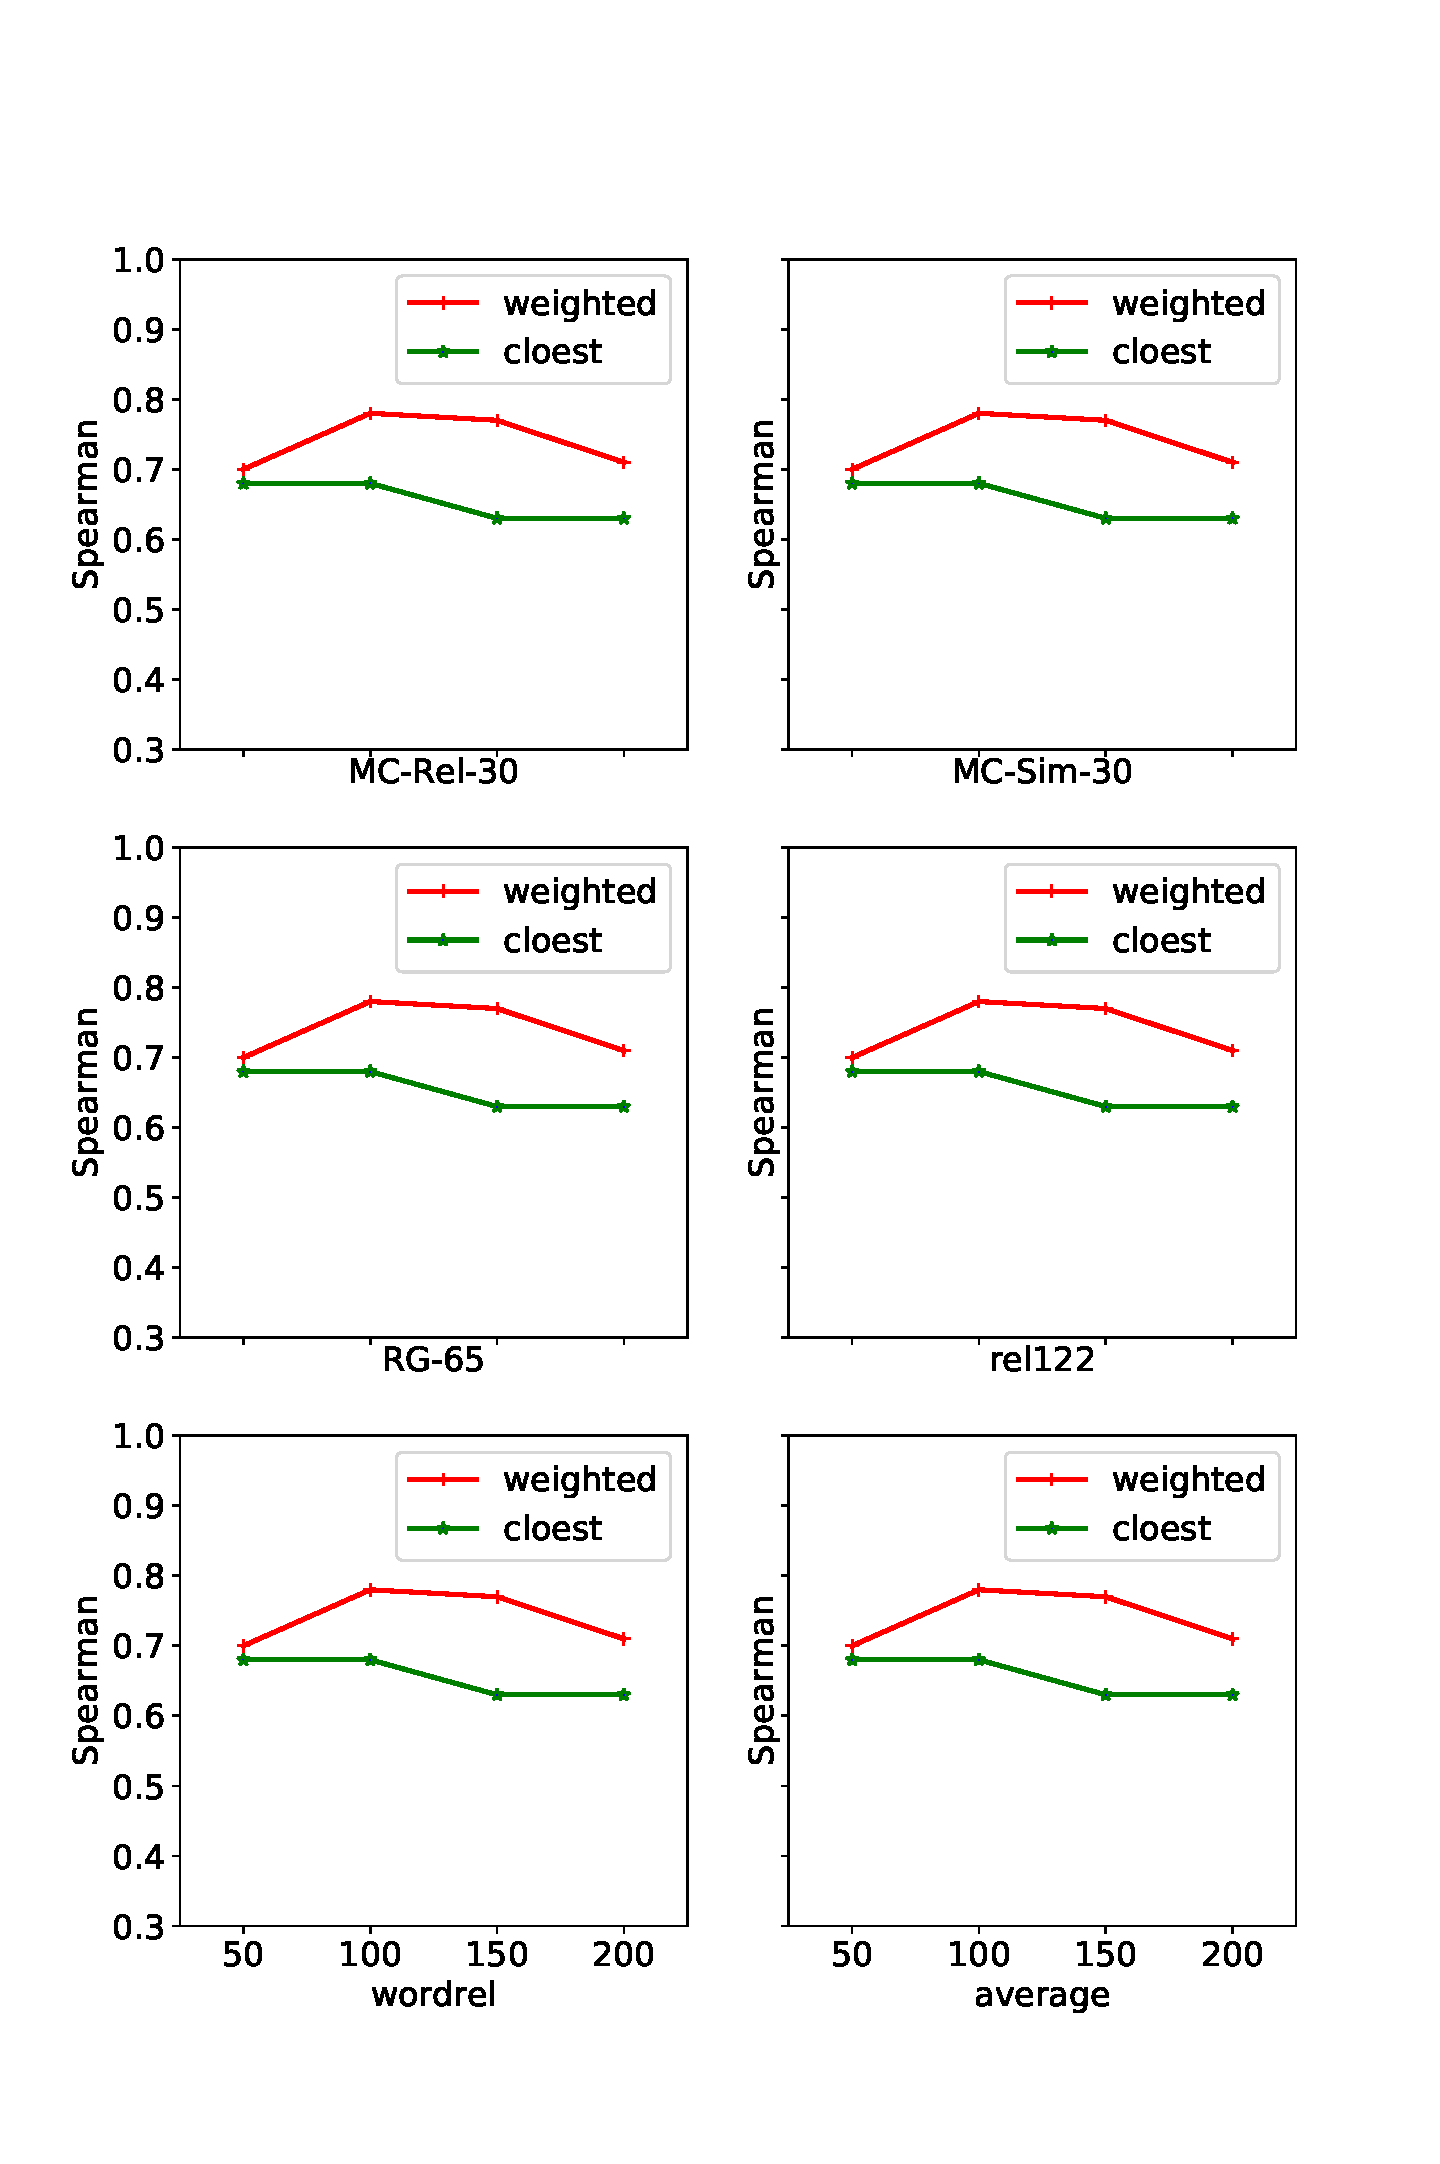
\includegraphics[width=55mm]{pic/dim.pdf}}
    \subfigure[The impact of the number of entities queried by given words]{
        \label{ent-num}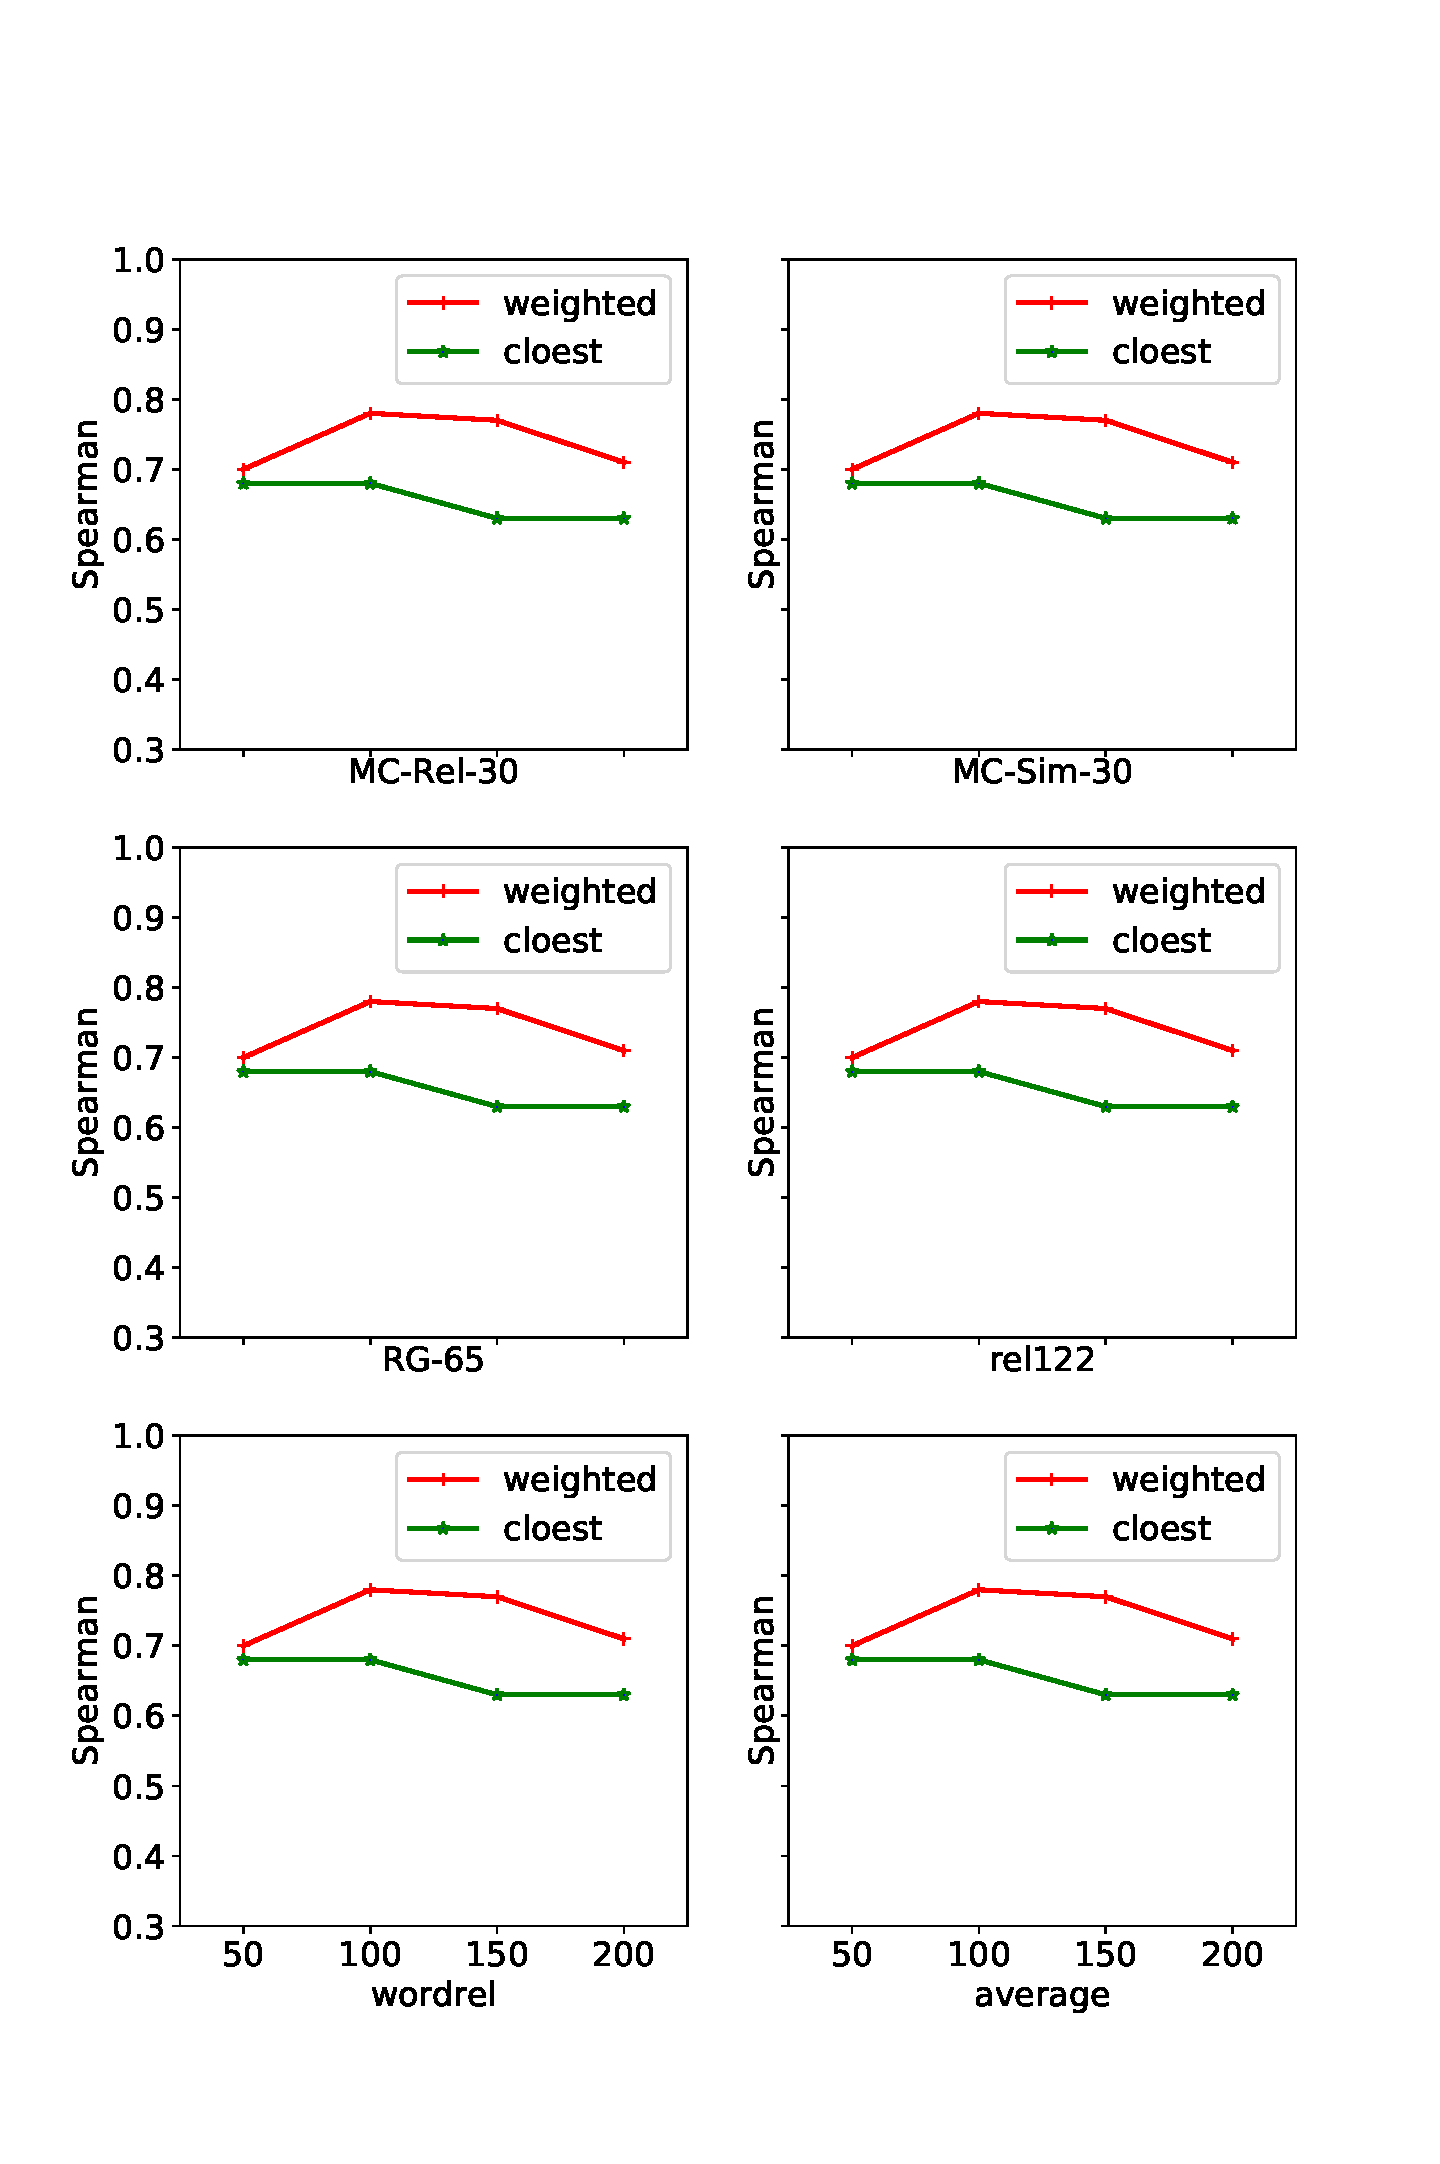
\includegraphics[width=55mm]{pic/dim.pdf}
    }
    \caption{Parameter Tuning}
\end{figure}


In the figure \ref{ent-num}, we draw the variation trend
of semantic relatedness scores following the increase of the quantity of entities queried by given words.
The slope of correlation coefficient curve rises gently with the increase of number of queried entities.
Distinguishingly, when the quantity of queried entities is greater than 5, the correlation coefficient
curve has a concave shown in pic \emph{X} because extra and overmuch entities would bring noise for the final
semantic relatedness scores.

\begin{table}[H]
    \centering
    \caption{Spearman correlation performance on five word similarity and relatedness datasets}
    \label{spearman}
    \renewcommand\arraystretch{1.15}
    \setlength{\tabcolsep}{2.5mm}{
        \begin{tabular}{lcllccl}
        \hline
        \multirow{2}{*}{\textbf{Measure}} & \multicolumn{5}{c}{\textbf{Dataset}}                                                                                          & \textbf{} \\ \cline{2-6}
                                        & \multicolumn{1}{l}{MC-rel-30} & MC-30 & RG-65                  & \multicolumn{1}{l}{rel122} & \multicolumn{1}{l}{wordrel} & Averrage  \\ \hline
        \textbf{WikiRelate!}              & --                            & 0.45          & 0.52                   & --                         & --                          &           \\
        \textbf{ESA}                      & --                            & 0.75          & 0.82                   & --                         & --                          &           \\
        \textbf{WLM}                      & --                            & 0.70          & 0.64                   & --                         & --                          &           \\
        \textbf{WikiWalk}                 & --                            & 0.61          & \multicolumn{1}{c}{--} & --                         & --                          &           \\
        \textbf{REWOrD}                   & --                            & 0.72          & 0.78                   & --                         & --                          &           \\ \hline
        \textbf{Pando-closest}            & \multicolumn{1}{l}{}          & 0.81          &                        & \multicolumn{1}{l}{}       & \multicolumn{1}{l}{}        &           \\
        \textbf{Pando-weighted}           & \multicolumn{1}{l}{}          & \textbf{0.85} &                        & \multicolumn{1}{l}{}       & \multicolumn{1}{l}{}        &           \\ \hline
        \end{tabular}
    }
\end{table}

Compared to previous method of semantic relatedness measurement, we run our model on five dataset
\emph{MC-Rel-30}, \emph{MC-Sim-30}, \emph{RG-65}, \emph{rel-122}, and \emph{WS-rel}, and report the
\emph{Spearman} correlation coefficient performance for the two strategies of our model. It can be
seen that our model proves to be highly reliable on semantic relatedness measurement tasks. Our model obtains
the best performance on most datasets. In addition, our approach in dataset \emph{MC-Rel-30} outperforms
the results in dataset \emph{MC-Sim-30} which proves that our model is more suitable for computing semantic
relatedness than similarity. 
\section{Conclusion}
test.

\bibliography{acl2018}
\bibliographystyle{acl_natbib}
\end{document}
